\documentclass[10pt]{beamer}
\usepackage[latin1]{inputenc}
\usepackage{amsmath}
\usepackage{amssymb}
\usepackage{graphics}
\usepackage{graphicx}
\usepackage{epsfig}
\usepackage{fancyhdr}
\usepackage{wasysym}
\usepackage{latexsym}
\usepackage{amsfonts}
\usepackage{subfigure}
\usepackage{color}
\usepackage[numbers]{natbib}
\usepackage{framed}
\usepackage{multirow}
\usepackage{booktabs}
\usepackage{chngpage}
\usepackage{caption}
\usepackage{tikz}
\usepackage{mdwlist}
\usepackage{algorithm,algorithmic,amsmath}



\DeclareMathOperator*{\argmax}{arg\,max}
\newcommand{\todo}[1]{\textcolor{red}{\textbf{TODO:} #1}}
\newcommand{\setD}{\ensuremath{\mathbf{D}} }
\newcommand{\setW}{\ensuremath{\mathbf{V}} }
\newcommand{\setC}{\ensuremath{\mathbf{C}} }
\newcommand{\matD}{\ensuremath{\mathrm{D}} }
\newcommand{\matW}{\ensuremath{\mathrm{W}} }
\newcommand{\matC}{\ensuremath{\mathrm{C}} }
\newcommand{\vecdi}[1]{\ensuremath{\mathrm{v}^{D}_{#1}}}
\newcommand{\vecwi}[1]{\ensuremath{\mathrm{v}^{W}_{#1}}}
\newcommand{\vecci}[1]{\ensuremath{\mathrm{v}^{C}_{#1}}}
\newcommand{\con}{$(w_{t-c}, \ldots, w_{t-1}, w_{t+1}, \ldots, w_{t+c})$}
\newcommand{\wgt}[1]{\ensuremath{\lambda_{#1}}}
\newcommand{\traindata}{\ensuremath{\mathcal{T}}}
\newcommand{\db}{\ensuremath{\mathcal{D}} }
\newcommand{\para}[1]{\noindent\textbf{%\fontsize{14}{15}\selectfont 
#1}} %{\paragraph{#1}}
\newcommand{\highest}[1]{\textbf{#1}}

\usetheme{Madrid}
%\usetheme{umbc1}
\title[{Distributed Document Representations for Multi-Label Document Categorization}]{Learning Distributed Document Representations for Multi-Label Document Categorization}
\author{\textbf{Nitish Gupta}}
\date{May 16, 2015}
\institute[IITK]{B.Tech - M.Tech Dual Degree\\
\vspace{.2cm}Thesis Defense\\ 
\vspace{.2cm}Electrical Engineering\\
\vspace{.2cm}IIT Kanpur }
\begin{document}
\setbeamercovered{clear}
%%%%%%%%%%%%%%%%%%%%%%%%%%%% 
\begin{frame}
\titlepage
%\begin{figure}[ht]
%\begin{center}
%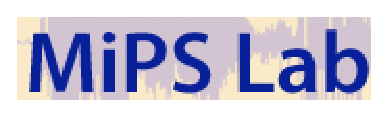
\includegraphics[width=1.75cm]{mips}
%
\epsfig{file=iitk_logo.eps,width=1.5cm}
%\end{center}
%\end{figure}
\begin{figure}[ht]
\begin{center}

\includegraphics[width=1.75cm]{iitk_logo-eps-converted-to.pdf}
%
\epsfig{file=iitk_logo.eps,width=1.5in}
\end{center}
\end{figure}
%\begin{figure}
%\begin{center}
%\hspace{-.0cm}
%\vspace{2cm}\includegraphics[width=1.25cm]{mips-eps-converted-to.pdf}
%\end{center}
%\end{figure}
\end{frame}

%%%%%%%%%%%%%%%%%%%%%%%%%%%%
\begin{frame}{Outline}
\begin{enumerate}
	\vfill\item Multi-Label Document Categorization
	\vfill\item Related Work
	\begin{itemize}
	  \vfill\item Text Representations
	  \vfill\item Learning Algorithms
	\end{itemize}  
	\vfill\item Distributed Word Representations
	\vfill\item Learning Distributed Document Represenations
	\vfill\item Document Cateogorization Algorithm
	\vfill\item Results
	\vfill\item Conclusion and Future Work
\end{enumerate}
\end{frame}

%%%%%%%%%%%%%%%%%%%%%%%%%%%%

\begin{frame}{Intoduction to Multi-Label Document Categorization}
\begin{itemize}
	\vfill\item<1-> Text Documents usually belong to more than one conceptual class. \\For E.g. an article on Music Piracy 
	\vfill\item<2-> Task of assigning documents to one or more predefined categories is called \emph{Multi-Label Document Categorization}
	\vfill\item<3-> Wide range real-world applications :
	\begin{itemize} 
	  \vfill\item<3-> Web-page tagging
	  \vfill\item<3-> Medical Patient Record Management
	  \vfill\item<3-> Wikipedia Article Management
	  \vfill\item<3-> Document Recommendation etc.
	\end{itemize} 
	\vfill\item<4-> Multi-label classification belongs to a general class of supervised learning algorithms where : 
	\begin{itemize}
	  \vfill\item<5-> Training instances in the form of document-category pairs are used to learn a classifier $\mathcal{H}$ 
	  \vfill\item<6-> Learned classifier $\mathcal{H}$ is used to assign categories to new test documents
	\end{itemize}
\end{itemize}
\vfill
\end{frame}

%%%%%%%%%%%%%%%%%%%%%%%%%%%%

\begin{frame}{Introduction to Multi-Label Document Categorization}
%\onslide<1->{ \textbf{Problem Statement}, } \\
\vfill\onslide<1->{ Given, }
\begin{itemize} 
	\vfill\item<1-> A set of documents $D = \{d_{1}, \ldots, d_{|D|}\}$
	\vfill\item<2-> A set of categories $C = \{c_{1}, \ldots, c_{|C|}\}$
	\vfill\item<3-> Training data for $n$ {\small ($n < |D|$)} documents, $\traindata = \{l_{d_{1}}, \ldots, l_{d_{n}}\}$ 
\onslide<4->{   \\ Each label vector $l_{d_{i}} \in \{0,1\}^{|C|}$ denotes relevance of categories to the document $d_{i}$ }
\end{itemize} 
\vfill
\onslide<5->{
	Example :
	\begin{table}[h!]
	\tabcolsep=0.1cm
	\tiny
	\begin{center}
	\begin{tabular}{c@{\hskip5mm} c c c c c c}
	\toprule
	\textbf{Documents}	&	\textbf{Sports} & \textbf{Music} & \textbf{Arts} & \textbf{Technology}  & \textbf{Literature} & \textbf{Politics}\\
	\cmidrule{1-1}
	\cmidrule{2-7}
	$d_{1}$ & 0 & 0 & 1 & 0 & 1 & 0\\
	$d_{2}$ & 0 & 1 & 1 & 0 & 0 & 1\\
	$d_{3}$ & 1 & 0 & 0 & 1 & 0 & 1\\
	$d_{4}$ & x & x & x & x & x & x\\
	$d_{5}$ & x & x & x & x & x & x\\
	\bottomrule         
	\end{tabular}
	\end{center}
	\end{table}
}
\vfill
\onslide<6->{
Using $\traindata$, $D$ and $C$ the learning algorithm learns a multi-label classifier $\mathcal{H}$ to estimate category label vectors, $l_{d_{j}}$ {\small $(j>n)$} for the test documents. 
}
\vfill
\end{frame}

%%%%%%%%%%%%%%%%%%%%%%%%%%%%

\begin{frame}{Introduction to Multi-Label Document Categorization}
\vfill\onslide<1->{ Document Categorization task has the following two components : }
\begin{enumerate}
	\vfill\item<2-> \emph{Learning Document Representations} : Representing text documents using numerical vectors that are inputs to the multi-label classifier $\mathcal{H}$
	\begin{itemize}
	 	\vfill\item<3-> Each document $d_{i} \in D$ is represented using a vector $v_{d_{i}} \in \mathbb{R}^{k}$ \\
	 	\vfill\item<4->	Vectors ($v_{d_{i}}$) should encode the semantic content of the documents 
	 	\vfill\item<5-> Encoding documents in a $k$-dimensional space using such represenation is called the \emph{Vector Space Model}
	 	\vfill\item<6-> The complete document set $D$ can be represented by a document representation matrix $\matD \in \mathbb{R}^{k \times |D|}$
	\end{itemize}
\suspend{enumerate} \vfill
\onslide<7->{	
\emph{ In this thesis, we focus on learning efficient document representations, $\matD$}	}
\vfill
	\resume{enumerate}
	\vfill\item<8-> \emph{Learning Algorithm} : Algorithm to learn the multi-label classifier $\mathcal{H}$
\end{enumerate}\vfill 
\end{frame}

%%%%%%%%%%%%%%%%%%%%%%%%%%%%

\begin{frame}{Background on Learning Algorithms}
\vfill
%\onslide<1->{ Learning algorithms can be classified into two classes :  }
\begin{enumerate}
	\vfill\item<2-> \emph{Learning Multiple Binary Classifiers} : \\
	\onslide<3->{ {\footnotesize	Algorithms that treat each category assignment independently and learn multiple binary classifiers, one for each category, to make the category assignments} 	} 
	\begin{itemize}
		\vfill\item<4-> Logistic Regression
		\vfill\item<5-> Support Vector Machines (SVM)
		\vfill\item<6-> Neural Networks
		\vfill\item<7-> Naive Bayes
	\end{itemize}

	\vfill\item<8-> \emph{Learning Single Joint Classifier} : \\
	\onslide<9->{ {\footnotesize	Algorithms that jointly assign all the categories to a document $d_{i}$, i.e. estimate the complete label vector $l_{d_{i}}$ using a single classifier} 	}
	\begin{itemize}
		\vfill\item<10-> k-Nearest Neighbor (k-NN)
		\vfill\item<11-> Linear Least Square Fit
		\vfill\item<12-> Decision Trees
		\vfill\item<13-> Generative Probabilistic Models
	\end{itemize}
\end{enumerate}
%\onslide<14->{ Learning a single joint classifier is usually better as it is able to exploit the category correlations }
\vfill
\end{frame}

%%%%%%%%%%%%%%%%%%%%%%%%%%%%%%

\begin{frame}{Background on Text Representation}
\vfill
\onslide<1->{
\textbf{Bag of Words Model} }
%Most common method to learn vector representations for a set of documents is the \emph{Bag of Words (BOW)} model 	}
\begin{itemize}
	\vfill\item<2-> Document $d_{i}$ represented by $v_{d_{i}} \in \mathbb{R}^{|V|}$
	\vfill\item<3-> Each element in $v_{d_{i}}$ denotes presence/absence of each word
	\vfill\item<4-> Weighing techniques employed to give importance to important terms
	\begin{itemize}
		\vfill\item<5-> Term Frequency (\emph{tf} )
		\vfill\item<5-> Inverse Document Frequency (\emph{idf} )
		\vfill\item<5-> Term Frequency - Inverse Document Frequency (\emph{tf-idf} ) : \emph{tf} $\times$\emph{idf}
	\end{itemize}
\end{itemize}
\vfill
\onslide<6->{
\textbf{Drawbacks of the Bag-of-Words model} }
\begin{itemize}
	\vfill\item<7-> High-dimensionality
	\vfill\item<8-> Sparsity
	\vfill\item<9-> Inability to encode word contexts
	\vfill\item<10-> Ignores word order
\end{itemize}
\vfill
% \todo{feature selection. Word Embeddings. Our document embedding. Our docu cate. Datasets. Results End}
% \vfill
\end{frame}

%%%%%%%%%%%%%%%%%%%%%%%%%%%%%%

\begin{frame}{Background on Feature Selection / Dimensionality Reduction}
\vfill
\onslide<1-> {
Techniques to deal with sparsity and high-dimensionality in BOW }
\begin{itemize}
	\vfill\item<2-> Information Gain \\
	\onslide<2->{ { \scriptsize
	\begin{equation}
	G(t) = -\sum_{i=1}^{|C|} P(c_{i})\log P(c_{i}) + P(t)\sum_{i=1}^{|C|} P(c_{i}|t)\log P(c_{i}|t) + P(\sim t)\sum_{i=1}^{|C|} P(c_{i}|\sim t)\log P(c_{i}|\sim t)
	\end{equation}
	} }
	\vfill\item<3-> Mutual Information \\
	\onslide<3->{ { \scriptsize
	\begin{equation}
	I(t,c) = \log \frac{P(t \wedge c)}{P(t) \times P(c)} \text{,}\qquad I_{avg}(t) = \sum_{i=1}^{|C|} P(c_{i})I(t,c_{i})
	\end{equation}
	} }
	\vfill\item<4-> Latent Semantic Indexing (LSI) \\
	\onslide<4->{ { \scriptsize
	\begin{equation}
	X = T S D^{T}
	\end{equation}
	} }
\end{itemize}
\vfill
\end{frame}

% %%%%%%%%%%%%%%%%%%%%%%%%%%%%%%

\begin{frame}{Distributed Word Representations}
%\vfill
\onslide<1->{
Representating each word $w_{i}$ using vector $v_{w_{i}} \in \mathbb{R}^{k}$ ($k \in [50, 300]$) } \\ \vspace{0.5cm}
\onslide<2->{
\textbf{ Need for Distributed Word Representations} } 
\begin{itemize}
	\vfill\item<3-> Curse of Dimensionality
	\begin{itemize}
		\vfill\item<4-> One-hot representations grow with the size of vocabulary
		\vfill\item<5-> Parameters in language modelling grow exponentially with the size of vocabulary
	\end{itemize}
	\vfill\item<6-> No Word Similarity Measure
	\begin{itemize}
		\vfill\item<7-> One-hot representations are orthogonal representations
		\vfill\item<8-> Cannot capture semantic similarity between words
	\end{itemize}
\end{itemize}
\vfill
\end{frame}

%%%%%%%%%%%%%%%%%%%%%%%%%%%%%%
\begin{frame}{Neural Probabilistic Language Model}
\vfill
\onslide<1->{
\citet{bengio2003neural} developed \emph{Neural Probabilistic Language Model (NPLM)} to learn}%learn distributed word vectors and a probability function that uses these vectors to learn a statistical model of language	}
\begin{enumerate}
\vfill\item<2-> Distributed word vectors
\vfill\item<3-> A probability function that, using these word vectors, learns a statistical model of language 
\end{enumerate}

\begin{columns}[T]
 \begin{column}{.5\textwidth}
 	\centering
 	\onslide<4->{
 	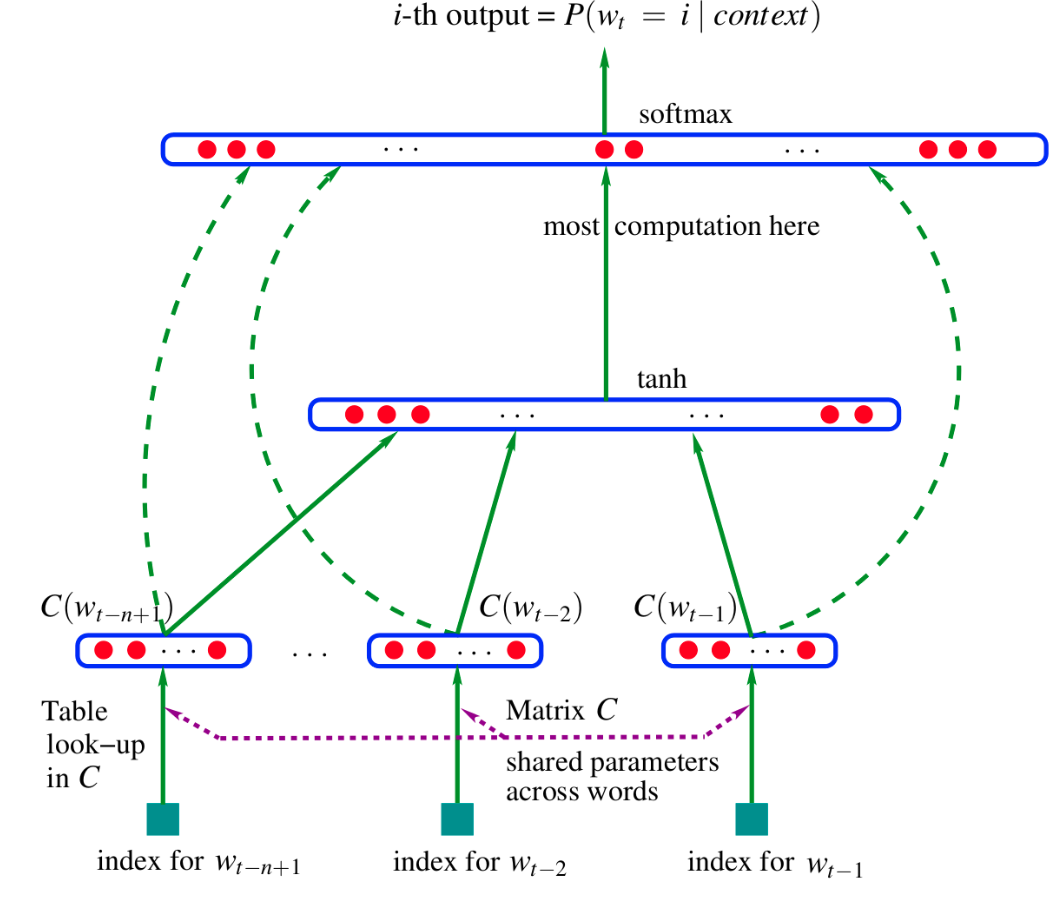
\includegraphics[scale=0.15]{../figs/bengio_nn.png} }

 \end{column}

 \begin{column}{.5\textwidth}
 	\centering
 	{\footnotesize
 	\vfill \onslide<5->{
 	\begin{equation}
    P(w_{t} | w_{1}^{t-1}) \approx P(w_{t} | w_{t-n+1}^{t-1})
    \end{equation} }
    \vfill \onslide<6->{
    \begin{equation}
	y = b + U tanh(d + Hx) \text{,} \quad y \in \mathbb{R}^{|V|}
	\end{equation} }
	\vfill \onslide<7->{
	\begin{equation}
	P(w_{t} = i | w_{t-1}, \ldots, w_{t-n+1}) = \frac{e^{y_{w_t}}}{\sum_{i}e^{y_{i}}}
	\end{equation} }
	}
 \end{column}
\end{columns}

\vfill
\end{frame}

%%%%%%%%%%%%%%%%%%%%%%%%%%%%%%

\begin{frame}{Log-Linear Models}
\vfill
\onslide<1->{
\emph{Log-Linear Models} for learning distributed word vectors are proposed in \citet{mikolov2013efficient}. These models use word vectors to predict other words in the context.	 }
% \begin{itemize}
% \vfill\item<2-> do not build a language model hence also consider future words in contexts
% \vfill\item<3-> show that the word vectors capture the semantic similarity between words
% \end{itemize}
\vfill
\begin{enumerate}
	\vfill\item<2-> Continuous Bag-of-Words Model 
	\begin{columns}[T]

	 \begin{column}{.5\textwidth}
	 	\centering
	 	\onslide<2->{
	 	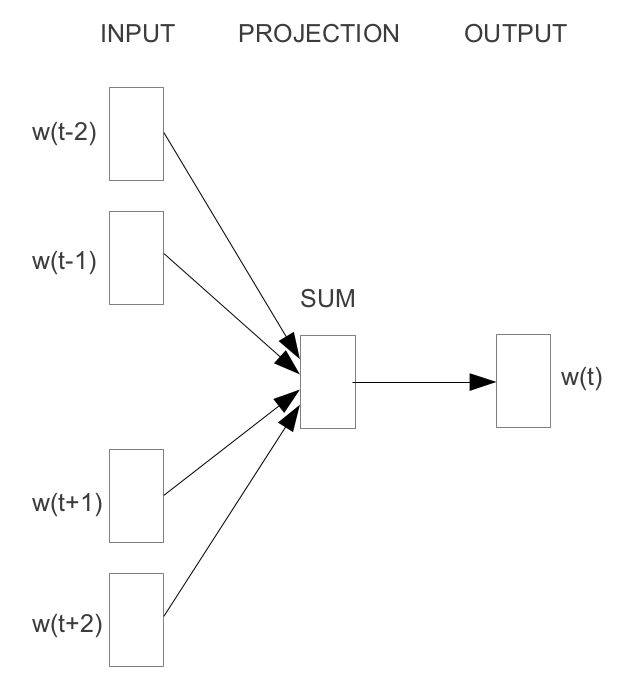
\includegraphics[scale=0.12]{../figs/mikolov_cbow.png} }
	 \end{column}
	 \begin{column}{.5\textwidth}
	 	\centering
	 	{\footnotesize
	 	\onslide<3->{
	 	\begin{equation}
	    h = w_{t-k} + \ldots + w_{t-1} + w_{t+1} + \dots + w_{t+k}
	    \end{equation} }
	    \onslide<4->{
	    \begin{equation}
		y = b + Uh \text{,} \quad y \in \mathbb{R}^{|V|}
		\end{equation} }
		\onslide<5->{
		\begin{equation}
		P(w_{t}|w_{t-k}, \ldots, w_{t+k}) = \frac{e^{y_{w_t}}}{\sum_{i} e^{y_{i}}}
		\end{equation} }
		}
	 \end{column}
	\end{columns}

	\vfill\item<6-> Skip-Gram Model
	\begin{columns}[T]

	 \begin{column}{.5\textwidth}
	 	\centering
	 	\onslide<6->{
	 	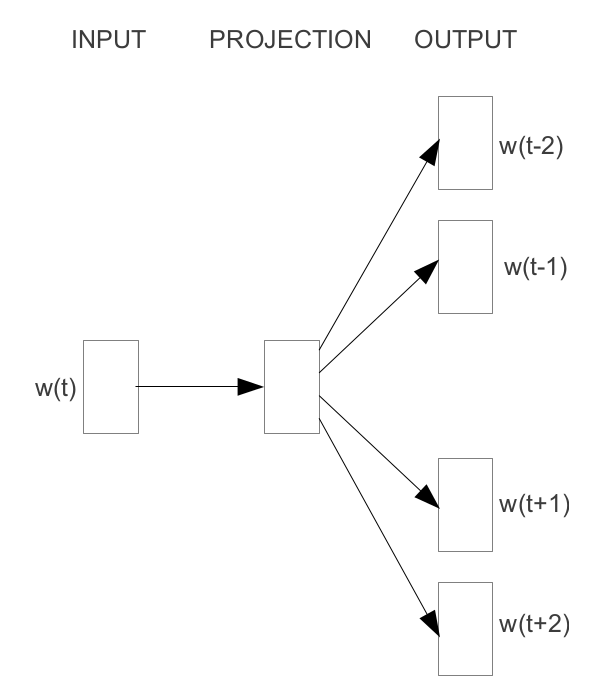
\includegraphics[scale=0.12]{../figs/mikolov_skip.png} }
	 \end{column}
	 \begin{column}{.5\textwidth}
	 	\centering
	 	\vfill
	 	{\footnotesize
	 	\onslide<7->{
	 	\begin{equation}
	    P(w_{t+j}|w_{t}) = \frac{e^{(v_{w_{t}} \cdot v_{w_{t+j}} )} }{\sum_{i} e^{(v_{w_{t}} \cdot v_{w_{i}})} }
	    \end{equation} }
	    }
	 \end{column}
	\end{columns}
\end{enumerate}

\vfill
\end{frame}

%%%%%%%%%%%%%%%%%%%

\begin{frame}{Distributed Document Representations}
\vfill \onslide<1->{
\textbf{Motivation for learning distributed document representations} }
\begin{enumerate}
	\vfill\item<2-> Traditional representations do not encode semantic similarity between documents. Therefore, cannot handle synonyms
	\vfill\item<3-> Drawbacks in BOW like sparsity, high-dimensionality, inability to encode context information and consider word ordering
	\vfill\item<4-> Compositionality of word vectors beyond weighted average \cite{mitchell2010composition, zanzotto2010estimating, yessenalina2011compositional, grefenstette2013multi, mikolov2013distributed} is not simple
	\vfill\item<5-> \citet{socher2013recursive} propose a Recursive Tensor Neural Network (RTNN) to compose word vectors for learning sentence representations using the parse-tree of the sentence in a bottom-up fashion
	\begin{itemize}
		\vfill\item<6-> Parsing, a computationally expensive step required for each sentence
		\vfill\item<7-> Composing sentence vectors to represent documents is not straight-forward
	\end{itemize}
\end{enumerate}
\end{frame}

% %%%%%%%%%%%%%%%%%%%%%%%%%%%%%%%%%%%%%%%%%%


\begin{frame}{Our Model for Learning Document Representations}
\vfill \onslide<1->{
\emph{Inspired by the log-linear models to learn word vectors, we present model, to learn universal distributed representations for documents and words } 
% \begin{quote}
% To learn universal distributed representations for documents and words
% \end{quote}
}
\vfill \onslide<2->{
\textbf{Hypothesis } 
\begin{quote}
Document Representations that encode semantic content of the document should be able to predict words in the document
\end{quote}}

\vfill \onslide<3->{
Our model, }
\begin{enumerate}
	\vfill\item<4-> Learns distributed representations for document (and words) that encode the different semantic content in the documents
	\vfill\item<5-> Embeds document and words in the same $k$-dimensional space such that semantically similar entities have similar vector representations
\end{enumerate}

%\begin{}

\end{frame}
% %%%%%%%%%%%%%%%%%%%%%%%%%%%%%%%%%%%%%%%%%%



% %%%%%%%%%%%%%%%%%%%%%%%%%%%%%%%%%%%%%
% \begin{frame}{Conclusions}
% \begin{itemize}
% \vfill\item The efficient method for modeling the pinna spectral notches over the median plane is discussed.
% \vfill\item The HRIR over the median plane are simulated by Fourier Bessel Series and reconstructed in a way that only highlights the pinna effect.
% \vfill\item The pinna spectral notches extracted from reconstructed HRTF are very smooth and accurate even at lower elevation angles as compared to those extracted from measured HRTF.
% \vfill\item The dimensions corresponding to pinna spectral notch frequencies when overlaid on ear contour show the high degree of resemblance to the actual pinna walls, when reconstructed HRTF are employed for the extraction of pinna spectral notches.
% \vfill\item Individual pinna spectral notches have been suggested for elevation angle perception to incorporate in HRTF when rendering the 3D audio. 
% \end{itemize}
% \end{frame}

% %%%%%%%%%%%%%%%%%%%%%%%%%%%%%%%%%%%%%
% \begin{frame}{Future Scope}
% \begin{itemize}
% \vfill\item Althought the relationship between ear morphology and pinna spectral notch frequencies has been established. Yet their is open issues regarding the depth and bandwidth of these notches.
% \vfill\item A strong pshchoacoustics argument need to be developed that relates the pinna anthropometry and depth and bandwidth of notch frequencies.
% \vfill\item The structural model of pinna has to be developed for the personalisatioon of HRTF according to individual ear shapes.
% \vfill\item It has been found that pinna spectral notches are perceptually very important for elevation angle. However, the pinna resonances are also significant in terms of perception.
% \end{itemize}
% \end{frame}
\begin{frame}{References}
    %{\footnotesize
    \bibliographystyle{abbrvnat}
    \bibliography{references}
    %}
\end{frame}


\end{document}